%
% The MIT License (MIT)
%
% Copyright (c) 2016 Paul Batty
%
% Permission is hereby granted, free of charge, to any person obtaining a copy
% of this software and associated documentation files (the "Software"), to deal
% in the Software without restriction, including without limitation the rights
% to use, copy, modify, merge, publish, distribute, sublicense, and/or sell
% copies of the Software, and to permit persons to whom the Software is
% furnished to do so, subject to the following conditions:
%
% The above copyright notice and this permission notice shall be included in
% all copies or substantial portions of the Software.
%
% THE SOFTWARE IS PROVIDED "AS IS", WITHOUT WARRANTY OF ANY KIND, EXPRESS OR
% IMPLIED, INCLUDING BUT NOT LIMITED TO THE WARRANTIES OF MERCHANTABILITY,
% FITNESS FOR A PARTICULAR PURPOSE AND NONINFRINGEMENT. IN NO EVENT SHALL THE
% AUTHORS OR COPYRIGHT HOLDERS BE LIABLE FOR ANY CLAIM, DAMAGES OR OTHER
% LIABILITY, WHETHER IN AN ACTION OF CONTRACT, TORT OR OTHERWISE, ARISING FROM,
% OUT OF OR IN CONNECTION WITH THE SOFTWARE OR THE USE OR OTHER DEALINGS IN
% THE SOFTWARE.
%

\section{Implementation}
\label{sec:implementation}

Now that we have looked at how the application is designed. In this next section we will go over the tools I used, how I went about implementing the features, and any problems that I came across along the way.   

\subsection{The tools}
\label{subsec:the_tools}

For this particular application I went with Java and JavaFX for the user interface and controllers. This meant right from the get go I had cross platform support. A MVC style architecture and with JDBC open access to SQL database connections. The only major issue was speed, as SQLite is known to be fast, whether my application could keep up with the requests that where being performed. However, as SQLite only allows one writer at a time this was never an issue. The other downside to using Java was not having direct access to the SQLite API through its own interface. But, after looking at the interface everything that I needed was supported through JDBC.

\subsection{The Modules}
\label{subsec:the_modules}

\subsubsection{The view and controllers}
\label{subsubsec:imp_veiw}

As previously mentioned, the architecture is MVC. And we are using JavaFX. JavaFX comes with a whole host of tools for working with the view, and controllers. 
\\\\
Firstly, each view or section can be represented using a fxml file. The fxml file is heavily based on HTML, including the support for CSS styling. Each file start with a root node, normally one of the panes. Such as border, anchor, and grid. For this application I stuck with anchor panes, apart from the menu bar which used a border pane. Then following the root pane is the items to attached to it. Each item can be given a unique id that allows it to be controlled with via Java and CSS. In addition to this you can include your own Java classes for custom items.
\\\\
Secondly, the controller is a normal Java class set as the controller for a particular fxml file. This can be done in two ways. The way is to inject the controller into the loading process. This allows you to call other code, such as initialisation before the fxml file is loaded, and keep track of the controller. The second way is to specify the controller inside the fxml file, and Java will load the controller in when the file is loaded. But you lose all access to the controller object. Inside the controller the annotation @FXML, allows Java to inject the item from the controller into the view, and vice versa. Giving you full control over the fxml file and object utilising the items unique id. Through my application I use the first method, to allow controller sharing, and manual control over the controller. 
\\\\
The view is made up of four sections, the menu bar, containing the file, edit and other drop downs, including the icons, and tabs. The other three section, represent the left, middle, and right sections of the central pane. This means that any one time I can display three different views. Each of the section have their own fxml file, depending on the situation they may also share a controller. This can be seen below in figure~\ref{fig:view_breakdown}.

\begin{figure}[H]
	\centering
	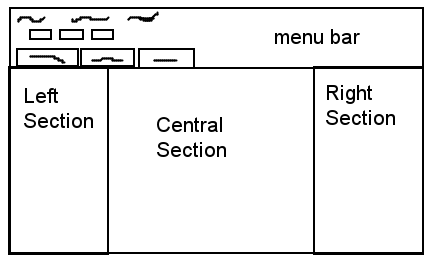
\includegraphics[scale=0.5]{images/view_breakdown.png}
	\caption{View breakdown}
	\label{fig:view_breakdown}
\end{figure}

I mentioned eariler that the menu bar will never change, and should never change. Using this fact the menu bar controller also doubles up as a 'master' controller. It controls what is currently seen in the other three sections. Loading and freeing up the necessary sections for that tab. 
\\\\
The central pane is a split pane, with two split dividers allowing each sections size to be adjusted on the fly to fit the users needs. If a section is not needed its just a matter of hiding that panes divider bar. 
\\\\
The controllers for each section extend a abstract controller class. The controller class, enforces a model interface object into the constructor, and implements Observer. The model interface allows each controller to separately contact the model, as previously mentioned to collect the data for the view. And by implementing observer we can register our controllers for the signal when the database is updated. Meaning we can collect the updated information as soon as it is ready. Without having to wait, or having a manual refresh button.    

\subsubsection{Model interface}
\label{subsubsec:imp_model_interface}

The model interface is based on a repository design with all the sub modules attached to it. In order for the controller to communicate with the sub modules they must also first go through the model interface. This design helps keep everything separated and compact. All of the sub modules attached to the model interface implement their corresponding interface. Allowing the implementation to change while keeping the same external view. This enables the design to be adapted to other systems other then SQLite. Below figure~\ref{fig:model_interface_design} show the layout of the model interface.

\begin{figure}[H]
	\centering
	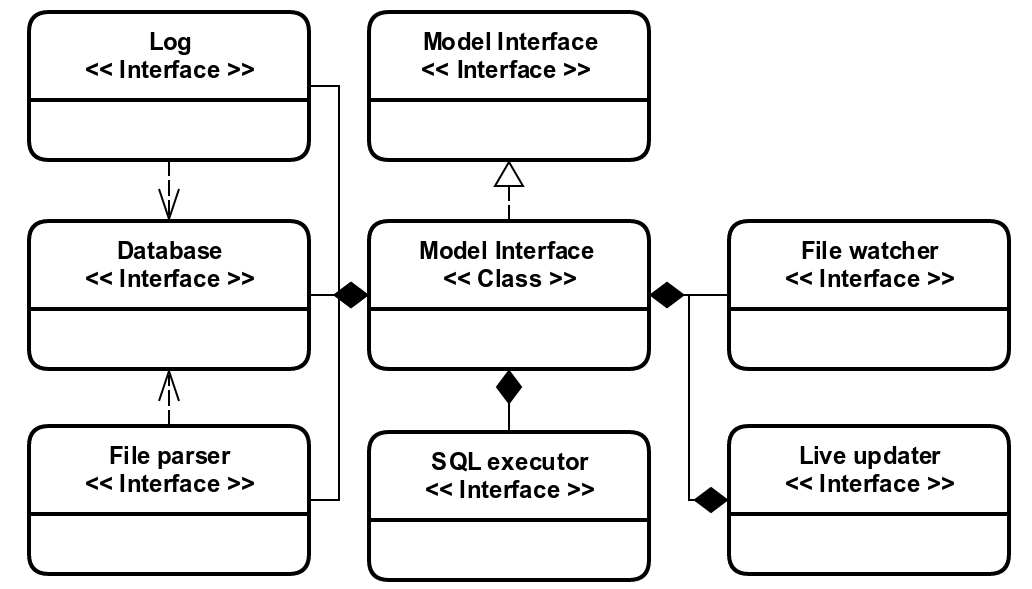
\includegraphics[scale=0.3]{images/model_interface_design.png}
	\caption{Model interface}
	\label{fig:model_interface_design}
\end{figure}

Everything is attached to the model interface, apart from the live updater being the exception with a copy of the model. In addition to providing access to the other modules, it has a very small amount of implementation, that is only used when every module is affected. Such as the case of setting up, closing and opening a database, which are all calls to the corresponding method on the modules interfaces. 

\subsubsection{The database}
\label{subsubsec:databse_imp}

The database module is made up of two parts, the interface and the storage. The interface controls access to the storage. Allowing the adding of new database items, retrieving of database items and stepping through the time line of database objects, and complete clearing of database items. Used with setting up and opening a new database, in order to make sure that the items are not mixed up with different files. The items are stored within a arraylist, and a int counter is used to keep track of where in the array we currently are.
\\\\
The storage is made up of database items, that contain a "snapshot" of the current state of the database file. The database item is made of two parts the meta-data, and B-Tree. The meta-data contains all the information in the header, including a few others such as number of tables, file name, and page number. The B-Tree is a custom implementation, holding the various B-Tree pages, as represented in the file. The database items are filled with information via the file parser. Out of all the classes, the database items, are the most used, being sent to the view for displaying, and modified by the various other modules during creation. 

\subsubsection{File watcher}
\label{subsubsec:file_watcher_imp}

In order to workout when the database was updated. I had two options, use SQLites API or watch the file. The API provided by SQLite is on a per connection base meaning that I would only revive signals when my own application sent SQL commands, which are of no use to me, as  I already know when the commands a sent out. This left me with the latter option, watching the file. Since SQLite is a single file, every time the file / database was updated so would the last modified time. In addition to this as SQLite only allows one writer at a time, I would revive a signal every update consistently.  
\\\\
The original implementation utilised Java's WatchService API. However, when I used it, I found it to be hit or miss whether it would register the change. At one point failed to detect any changes. In the end I ended up rolling my own solution, which is a simple while true loop, recording the last modified time, then when the time differs we send out a single to the rest of the application. 
\\\\
Due to the polling nature of this module, it runs inside its own thread, and communicates over an observer patten, that any another class can tune into, providing they implement the Observer interface. The thread could then process the updated databases without stopping or slowing down the user interface and other interactions.

\subsubsection{File parser}
\label{subsubsec:file_parser_imp}

The file parser takes a database file, a database object, and converts the database file into the databse object. Parsing the database, starts with checking the magic number, then the header, before moving onto the pages. The magic number and header information is just reading the first 100 bytes, correctly. For the pages I relied heavily upon recursion.
\\\\
First I would parse the page header, then switch into the method, that dealt with that type of page, who would then call the original method, when it reached a page number.  Each page was represented as a node, with with contents of the node represented as a cell. The only main issue with this design is the size of the stack on a large database. Below is the psudocode of the algorithm:

\begin{lstlisting}	
public void parseBTree(stream, database) {
	database.getBTree().setRoot(parsePage(stream, 1, 
								database.getPageSize()));
}

public Node parsePage(stream, pageNumber, pageSize) {
	Node node = new Node();
	PageHeader header = parseHeader(stream, pageNumber, pageSize);
	
	BTreeCell cell;
	switch(header.getType()) {
		case (TABLE_BTREE_LEAF_CELL) {
			cell = parseTableBtreeLeafCell(stream, pageNumber, 
											pageSize);
		}
		....
	}
	if (header.getType() == INTERIOR_CELL) {
		node.addChild(parsePage(in, pageHeader.getRightMostPointer(), 
						pageSize));
	}
	node.setData(cell);
	return node;
}

public cell parseTableBtreeLeafCell(InputStream, PageHeader, Node) {
	Cell cell = new Cell();
	
	int cellPointers[] = header.getCellPointers();
	foreach(cellpointer) {
		cell.data = readData();		
		if (cell has pageNumber) {
			node.addChild(parsePage(in, pagenumber, 
						pageSize));
		}
	}
	
	return cell;
}
\end{lstlisting}

During the process of parsing the tree we also need to decode the 'varints' mentioned in section~\ref{subsubsec:sqlite_data_encoding} especially as we needed to count the number of bytes for the record headers. Below shows the psudocode algorithm that I made in order to decrypt them: 

\begin{lstlisting}	
private long[] decodeVarint(stream) {
	long[] value = new long[];
	byte[] varint = new varint[9];
	
	for (i = 0 to 9) {
		varint[i] = stream.readByte();
		if (first bit is not set) {
			break;
		}
	}
	
	if (i == 0) {
		value[0] = 0;
		value[1] = 1;
	} else {
		for (j == 0 to i) {
			varint[j] = (varint[j] << 1);
		}
		value[0] = varint.toLong();
		value[1] = i + 1;
	}
	return value;
}
\end{lstlisting}

The first value returned in the array is the value of the varint, and the second its size. 

\subsubsection{The log}
\label{subsubsec:log_imp}

The log, though the project has under gone many design changes. The original plan was to have the log run on its own without having to relay on other modules, and would retrieve the original SQL commands that were sent to the database. However, as we we will see, this proved unattainable, and I had to only record the changes that occure when a command is sent. While working on the log there were three ways I could have implemented it in addition to my final method.
\\\\
The first technique I looked at utilised SQLites triggers. Triggers execute SQL commands when, a Delete, insert or update is performed on a table, with a optional where clause. Using this \cite{sqlitetriggers} used three separate triggers to long the time, changes before and after, and type of action performed on the table. The last part is one of the reason why I went for another technique. Firstly, I would need to have three triggers per table in the database, so N*3 triggers where N is the number of tables. Secondly, in order to accomplish this, I needed my own table that the changes are stored to, hence the log file in my original design, where I would attach to the database and write to it. lastly, the triggers meant altering the database file, this is something I wanted to avoid as much as possible, as to not imped on the running of the database.  
\\\\
The second solution, was to try and hook into SQLite through its API more specifically the sqlite3\verb|_|trace function. You pass it a callback function, that is called with the SQL commands, at various stages as it passes through the system. Unfortunately for me at the current time the JBDC for SQLite did not support the function that I needed. So I ended up writing a couple C functions that I could then call from Java in order to access the API. It worked for the most part, apart from that method only calls the callback function for SQL sent from the current application. When I needed to collect all the changes, thus make this unusable. 
\\\\
The third way was to write my own extension to SQLite, or download the source code, and modify to suit my needs it. The seemed to be way to far from the original path, and if I used a custom version it meant that it would be limited to only my version of SQLite. And as mentioned previously, I wanted to not modify the data if possible, so writing an extension, that would have to be loaded into SQLite and attached to the database, possibly conflicting with any other extensions they might have.
\\\\
The final option, while less sophisticated then the others, works well, although I do not get the original requests. I do end up recording the time, and all changes that happened per command. Since the database storage contains all of the previous versions like a snapshot of the database. when a update comes in I simply compare the new updated database to the last database object that passed through the application.
\\\\
In order to compare database required looping through every data value in both trees and comparing them, not only the data values, but also the added and removed pages. This could not be detected through any of the other techniques. Clearly looping through every single item in a larger database would quickly become a bottleneck, and slow the application and parsing down. So in order to speed it up, I did two things, firstly hashed the data array, If the hashes matched then we do not have to loop through the data. The second this was to adjusted my B-trees into a modified version of the Merkle Tree by \cite{merkletree}. The basic idea behind the merkle tree is that each node in the tree has a hash of its children’s hash, all the way down to the leaf node, who’s hash is based on the contents. Below figure~\ref{fig:merkle_tree} shows a digram of the merkle tree.

\begin{figure}[H]
	\centering
	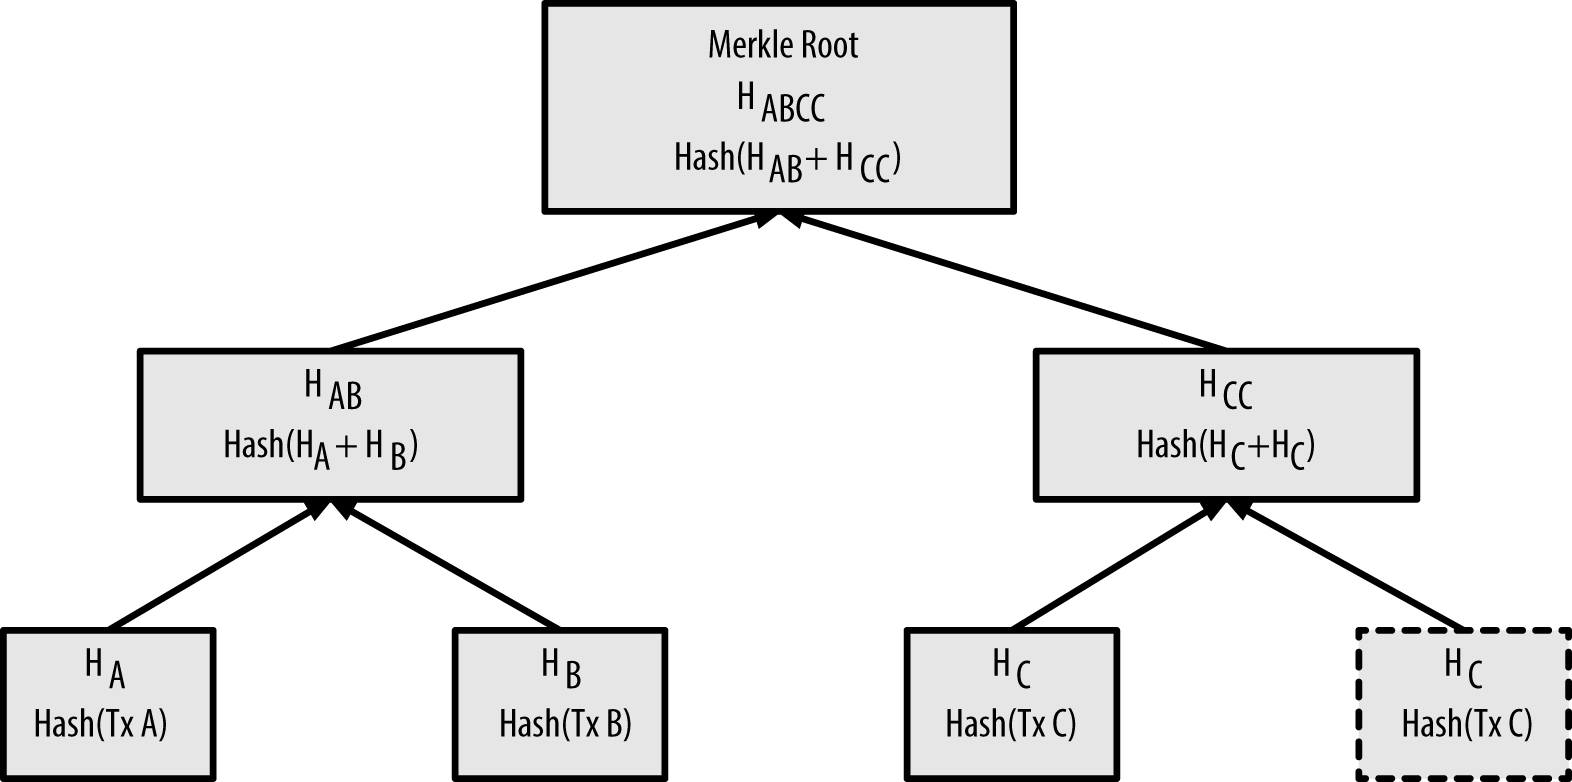
\includegraphics[scale=1.0]{images/merkle_tree.png}
	\caption{Node hashes in a  merkle tree \citep{bitcoin}}
	\label{fig:merkle_tree}
\end{figure}

With this we can tell if there is any change in the current section of the tree just by comparing the nodes hashes without having to loop over them, allowing the program to only loop over the nodes when a change is detected. Otherwise we can skip it. Unless the entire database is modified, where we will have to revert to looping over everything. The hash for each node is calculated off the hash of the data inside it, and its children’s data. This will tell us if a page has been added, removed or modified. 
\\\\
When it detects an update to the data, it will mark that page as modified, a simple boolean value. Recording the string value, from the old page and new page, into a log object. If instead it was a removal or addition, of data, it will store the new / removed value. Something similar happens with added and removed pages. With the addition of pages, the added page will be marked as changed. Often when this happens a pointer to the new page will also be placed somewhere, so this is also recorded. When a  page is removed, utilising the data from the old tree we can see exactly what was page has been removed and can record it, but there is nothing to marked as changed, apart from the pointers in other pages to that page. 

\subsubsection{Live Updater}
\label{subsubsec:live_Updater_imp}

The Live updater has undergone many changes from the start, although its position in the architecture has not changed, it gradually was morphed and shaped by the rest of the application. Originally it stared out as a module that would control the parsing of the application. By contacting the database and telling it when to move along the time line, allowing the pausing of live updates. It would also receive the update signal from the file watcher, and parse the file, moving it into the database storage. Basically an extra more controlled, and tailored interface into the database interface linking it to the file parser.
\\\\
However, to collect metadata information about the database, I had to run SQL onto the database, else I would have to loop through the entire tree again. So it needed access to the SQL executer, which we will cover in the next section. Then I ran into problems with the log feature, and while working a way around the problem, it ended up iside this module. As a result of this the module soon became bloated, as I added new features, since this was the only module that had access to all the needed resources.
\\\\
Rather fighting against my designs I decided it would be better to dedicate this as a master module, that would orchestrate the process when an update signal is revived. This allowed me to move the extra jobs it had taken on back into their correct modules, as a result of this it does exactly what I said in the beginning. Acting as a tailored interface into the database interface, contacting the file parser, SQL executor, and Log modules to control the parsing of the updated database.
\\\\
When an update signal is received, it requests a database object from the file parser, and add the extra metadata from the SQL command. It then requests the previous database object from the database interface, and send them to the log. Before storing the new database object inside the database interface. If we are not paused it will then increment along the time line. 

\subsubsection{SQL executor}
\label{subsubsec:sql_executor_imp}

The SQL executor manages the JDBC connections to the database, making sure that it connects, closes and commits any changes that are needed onto the database. Its interface provides four methods to the other modules, connect, close, perform select, perform update and get database metadata. Unlike the rest of the modules this was one of the more straight forward and simple to implement, calling the corresponding functions on the JDBC.

\subsection{User Interface}
\label{subsec:user_interface_imp}

I mentioned in the last section how the view is put together, but now we have looked at each of the modules in turn. I wanted to go through how each of the different tabs / features are put together. In order to better understand how each module is interacted with.
\\\\
The entire user interface is made up of eight fxml files and one CSS file, for styling. As mentioned previously, the fxml files contain the layout for each of the sections. I opted for a dark colour scheme used through out the application, due to personal preference, however this could easily be swapped out for a lighter version. 
\\\\
The menu bar is made up of one fxml file. In addition to the visual elements using the JavaFX key code combination class, I proved keyboard short-cuts such as 'control o' to open a database, and 'control-q' to quit. The controller for this fxml file  contacts the model interface for the opening and closing the database, and the live updater for controlling the time line.  This can be seen below in figure~\ref{fig:ui_screen}.

\begin{figure}[H]
	\centering
	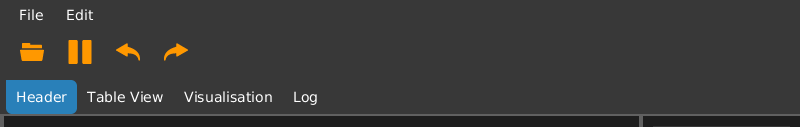
\includegraphics[scale=0.32]{images/ui_screen.png}
	\caption{Menu bar.}
	\label{fig:ui_screen}
\end{figure}

The right section is made up of a single fxml file, containing the SQL executer. As previously mentioned the SQl executor module enables arbitrary SQL commands to be ran on the database. As such this section contacts the SQL executor in order connect, run commands, and close the connection. This final interface can be seen below in figure~\ref{fig:ui_imp_sqlexe}.

\begin{figure}[H]
	\centering
	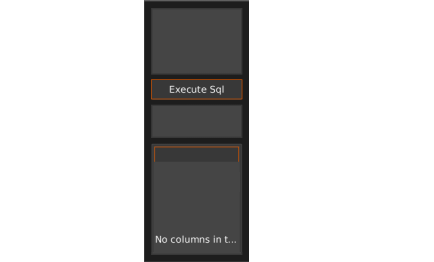
\includegraphics[scale=0.7]{images/ui_sqlexe_design_final.png}
	\caption{SQL executor UI.}
	\label{fig:ui_imp_sqlexe}
\end{figure}

The meta data tab is made up of single fxml file. The outer layer is a scroll pane, with a flow plane content. The flow pane provides a dynamic layout to adjust to different resolutions alongside the scroll pane. The panels, inside of the flow pane are pane with grid pane content. The grid pane is has two columns. The left or first column, representing the description or name and the right or second column the value. In order to collect the meta data, the controller needs to contact the database interface, to collect the current database object. The user interface can be seen below in figure~\ref{fig:ui_imp_metdata}.

\begin{figure}[H]
	\centering
	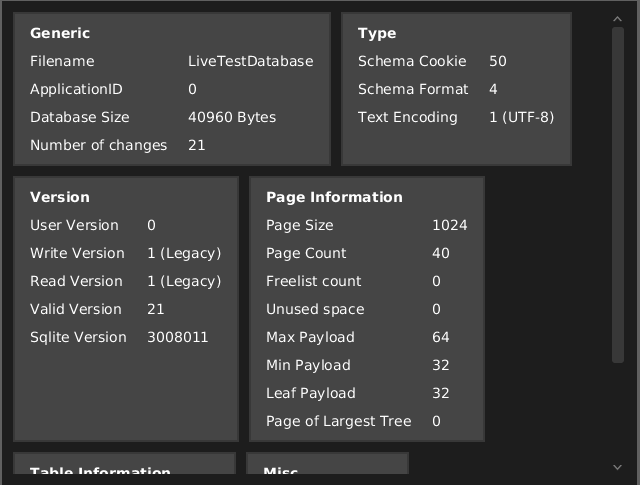
\includegraphics[scale=0.32]{images/ui_meatadata_final.png}
	\caption{Metadata UI.}
	\label{fig:ui_imp_metdata}
\end{figure}

The table view is made up of two fxml files that share a controller. The table view allows user to select a  table and view the schema and all the data within it. In order to accomplish this it contacts the SQL executor, and runs a select all query to collect the data, and a select from 'sqlite\verb|_|master' to retrieve all tables and schemas. This interface can be seen below in figure~\ref{fig:imp_ui_table}.

\begin{figure}[H]
	\centering
	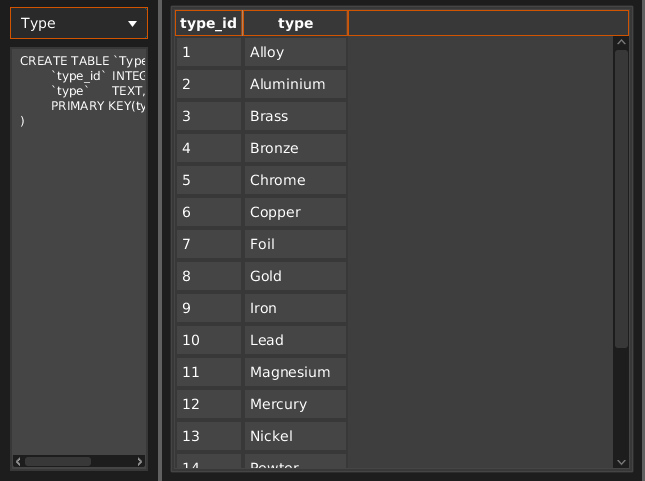
\includegraphics[scale=0.32]{images/ui_table_final.png}
	\caption{Table view UI.}
	\label{fig:imp_ui_table}
\end{figure}

The visualiser is made up of two fxml files, sharing a single controller. The center section containing the visualisation of the database, uses a custom scroll pane node to enable, zooming in addition to scrolling. Each node is represented as a pane, with a CSS class for the colouring. The node, contains the corresponding B-Tree node, from the database object. This is then used to display the data within the left side pane. In order to draw the structure I first sort out the horizontal position going top down. This is also used to load the nodes, via recursion. After all the nodes are loaded I then caclutate the horizontal positions on a second pass through bottom up. This interface can be seen below in figure~\ref{fig:improvised}.

\begin{figure}[H]
	\centering
	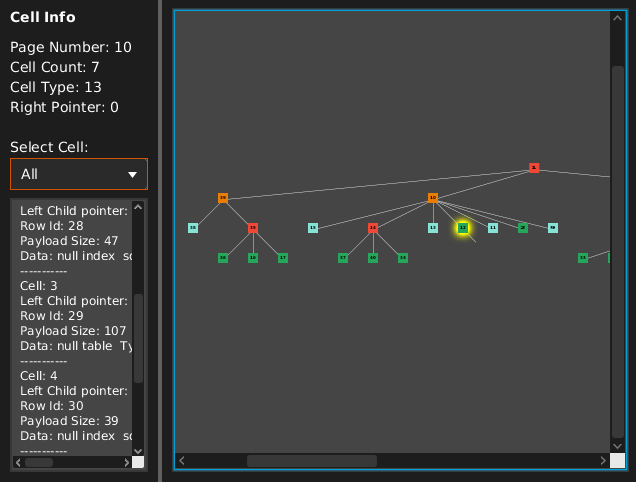
\includegraphics[scale=0.32]{images/ui_visuliser_final.png}
	\caption{Visualiser interface design.}
	\label{fig:imp_ui_vis}
\end{figure}

The log, is made up of one fxml file. Similar to the meta data tab, it contains a single scroll pane, with a VBox inside. allowing it to contain infinite items. Each item is made up of a Titled pane. Where the title is the time and data of the update, and the content, the changes that where performed in the update. To collect the data, it contacts the Log module, and receives a list of log items. This can be seen below in figure~\ref{fig:imp_ui_log}.

\begin{figure}[H]
	\centering
	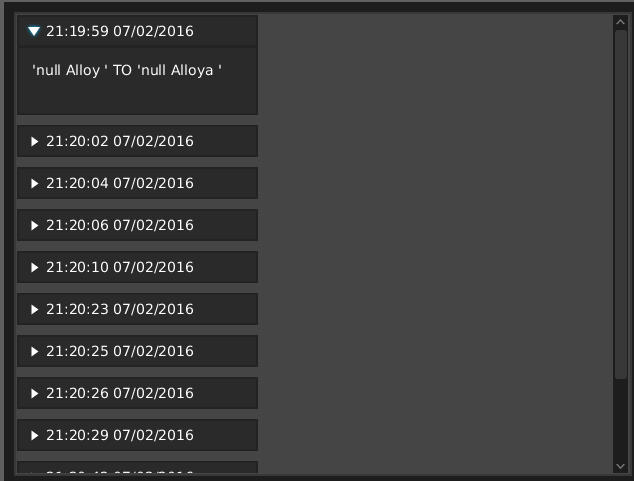
\includegraphics[scale=0.32]{images/ui_log_final.png}
	\caption{Log UI.}
	\label{fig:imp_ui_log}
\end{figure}
